\documentclass[a4paper,oneside,1pt]{article}
\usepackage[utf8]{inputenc}
\usepackage[T1]{fontenc} 
\usepackage{hyperref}
\usepackage{amsmath,amssymb}
\usepackage{fullpage}
\usepackage{graphicx}
\usepackage{url}
\usepackage{xspace}
\usepackage[french]{babel}
\usepackage{multicol}
\usepackage{geometry}

\usepackage[utf8]{inputenc}

\geometry{hmargin=2.5cm,vmargin=1.5cm}

\title{TP NoSQL - Neo4J}
\author{DANTIGNY Raynald - DE GEA Jordan - DUCLOT William}

\begin{document}

%You have to provide a compressed file that contains the report and two folders:
%- Folder 1 contains the data, scripts and instructions to populate the database.
%- Folder 2 contains the queries proposed (one file by query)

%The compressed file name must follow the next format: “noSQL_MSBigData_GroupXX”, where XX have to be changed by the corresponding number group assigned by Teide.

%Write a text describing the data stored in the database. This text should not exceed 15lines.You can include a figure to illustrate.

% Text font size: 11 or 12


\maketitle

\section{Introduction}

\subsection{Technologie and choix de sujet}
On savait que MongoDB était plus tilisé que Neo4j (par exemple pour les backends mobiles). C'est pourquoi on a préféré utiliser Neo4j: parce que ce TP est une opportunité pour nous de créer et utiliser une base de donnée Neo4j. De plus, on a choisi Neo4j car les applications dans le cadre de ce projet nous semblaient plus intéressantes.
\linebreak

Notre sujet se nomme "Pronostique des listes gagnantes d'un école". On voulait donc profiter de ce TP pour mettre en place une application concrète. L'objectif est de prédire les listes gagnantes d'une campagne d'élection au BDE, BDS, BDA... En bonus, nous allons pouvoir calculer les budgets, et les gains de chaque liste (notamment avec les sponsors, les soirées organisées, etc...). 

\subsection{Utilisation}


Pour remplir la base de donnée, le fichier \texttt{generate.php} nous permet de générer des données aléatoires. La sortie de ce script doit être redirigée directement dans un fichier (dans le cas où vous n'avez pas php, un fichier data.txt est fourni):

\texttt{php generate.php > data.txt}

La base de donnée peut être initialisée avec ces données: dans le dossier d'installation de neo4j, exécuter la commande:

\texttt{./bin/neo4j-shell -file [path\_to\_data.txt] -path ./data/databases/graph.db}

\section{Projet}

\subsection{Base de donnée}

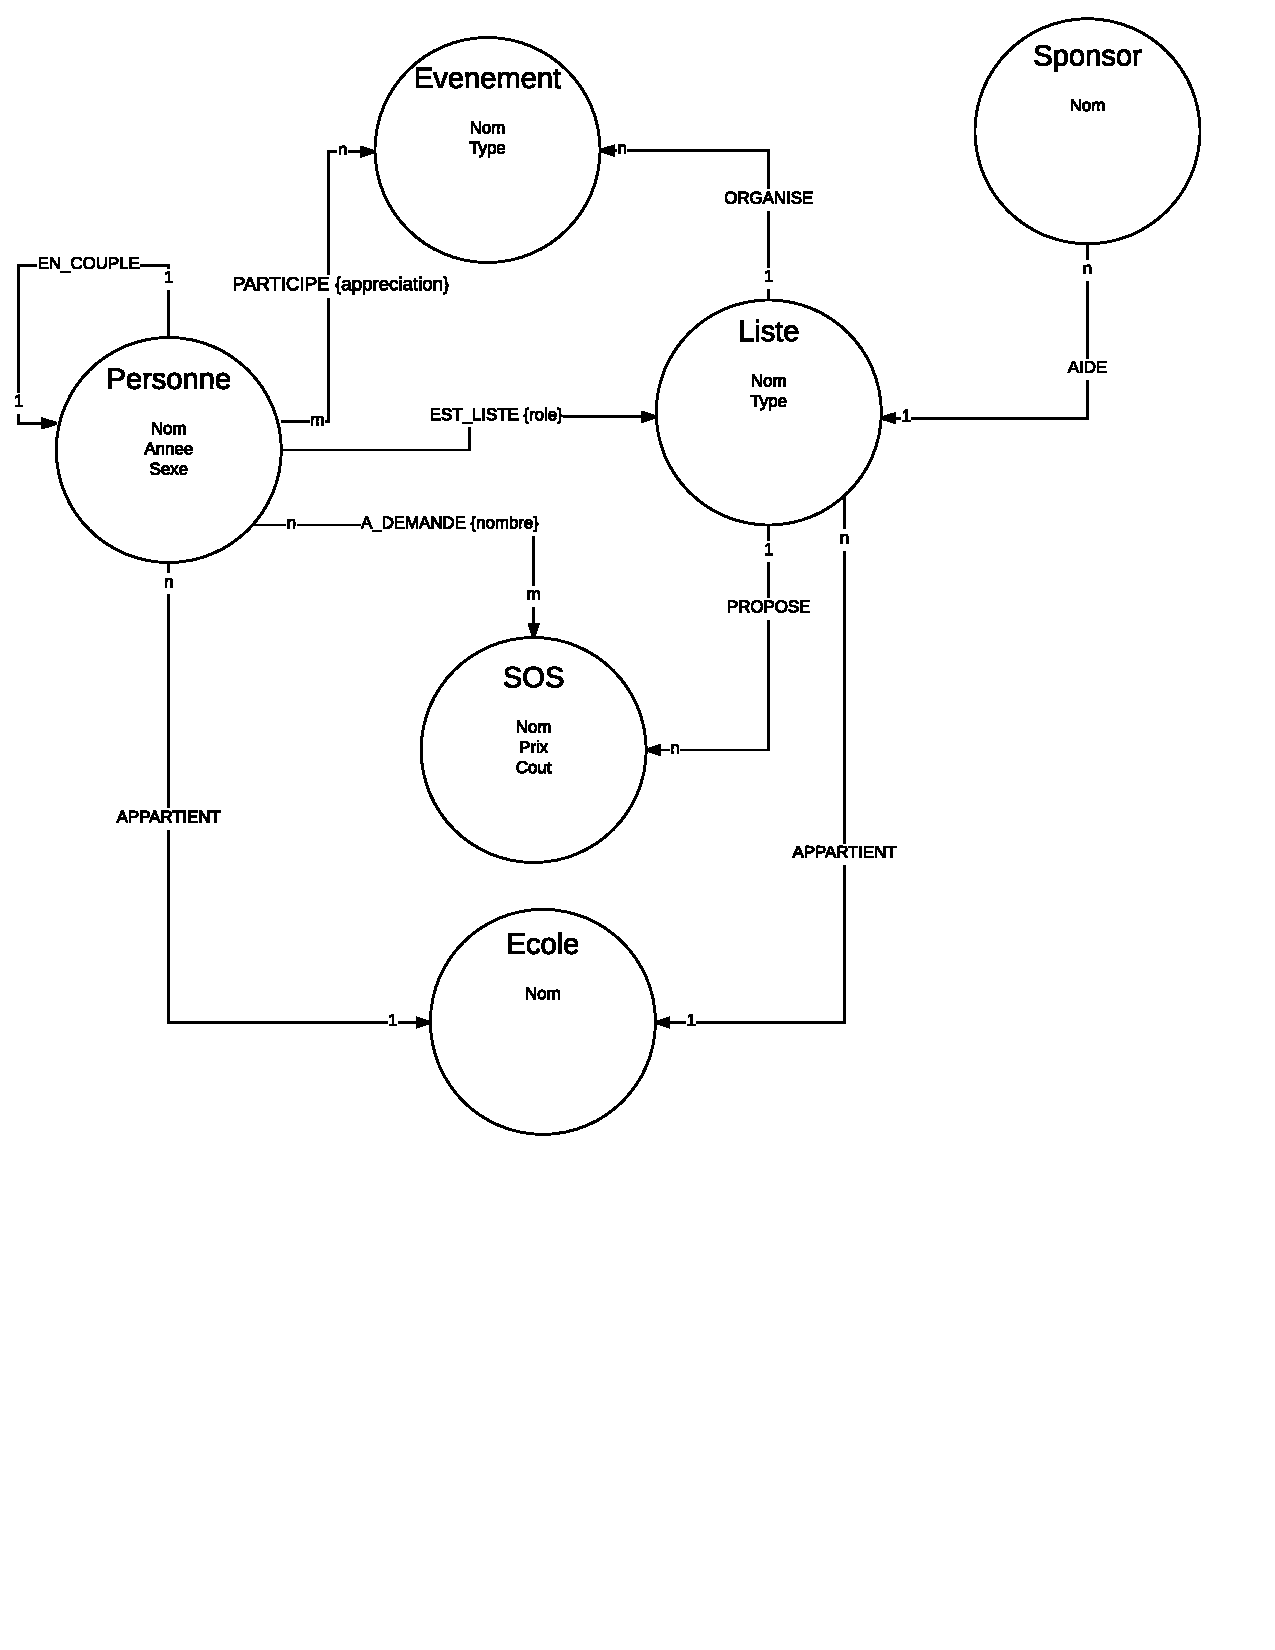
\includegraphics[width=18cm,trim = 0cm 8cm 0cm 0cm, clip=true]{schema.pdf}

Chaque \textit{Liste} peut proposer différents \textit{SOS}.  \\
Chaque \textit{Liste} peut proposer différents \textit{Evenement}.  \\
Chaque \textit{Personne} peut être en couple avec une autre \textit{Personne}. \\
Chaque \textit{Sponsor} peut aider une seule \textit{Liste}. \\
Un nombre défini de \textit{Personne} (ex 25) peut être dans une \textit{Liste}. \\
Chaque \textit{Personne} peut demander différents \textit{SOS} à différentes \textit{Liste}. Ils peuvent demander plusieurs fois le même \textit{SOS}. \\
Chaque \textit{Personne} peut participer à plusieurs \textit{Evenement}. \\
Chaque \textit{Personne} est dans une seule \textit{Ecole}. \\
Chaque \textit{Liste} est dans une seule \textit{Ecole}. \\
\subsection{Index}
\subsubsection{Index sur les noms}
Afin de sélectionner une personne par son nom plus rapidement on crée l'index suivant.
\\
\begin{verbatim}
CREATE INDEX ON :Personne(nom);
\end{verbatim}
\subsubsection{Index sur les rôles}
Afin de sélectionner une personne listée par son rôle plus rapidement on crée l'index suivant.
\\
\begin{verbatim}
CREATE INDEX ON :EST_LISTE(role);
\end{verbatim}
\subsection{Requêtes}

% Liste des requetes
% 1 file by query
% Describe the indexes proposed and explain yourdecision.This text should not exceed 4linesby index.
% For each query, provide it :
%   in natural language.  This text should not exceed 3 lines
%   in the language of the systemand
%   If there are indexes involved, describe their impact. This text should not exceed 3linesby index
%   Advantages and disadvantages of the query implementation proposed.

\subsubsection{Requête 0}
Cette requête permet de tester l'efficacité de l'indexation. On a donc indexé les personnes par leur nom.
\\
On veut sélectionner toutes les participations de la personne qui a pour nom "Nom14". 
\\
\begin{verbatim}
MATCH p = (:Personne{nom:"Nom14"})-[:PARTICIPE]-() RETURN p
\end{verbatim}
\\L'indexation permet de directement sélectionner le nœud de la personne sans parcourir tous les noeuds de type Personne.

\subsubsection{Requête 1}
Retourner pour chaque liste son type (BDA, BDS, BDE), son président et son école.
\\
\begin{verbatim}
MATCH (l:Liste)-[:APPARTIENT]->(e:Ecole)
MATCH (p:Personne)-[:EST_LISTE {role:'president'}]->(l)
RETURN l.nom,p.nom,e.nom
\end{verbatim}

Pour accélérer la requête, on a créé un index sur le rôle de chaque listé, ainsi c'est plus rapide de trouver le président car il y en a qu'un seul et on a donc pas à parcourir tous les nœuds pour le trouver.


\subsubsection{Requête 2}
Calculer pour chaque liste la somme totale obtenue par ses sponsors
\\
On selectionne chaque relation liste/sponsor. Puis pour chaque liste, on additionne les montants des aides.
\\
\begin{verbatim}
MATCH (l:Liste)-[a:AIDE]-() 
RETURN l.nom, sum(a.montant) AS Subventions
\end{verbatim}
\\
La requête est courte donc facilement lisible. Elle a en revanche le désavantage de ne pas avoir de clause GroupBy explicite comme en SQL.

\subsubsection{Requête 3}
Retourner les couples dont un des membres est dans plus d'une liste.
\\
Ici on prend d'abord tous les couples. Ensuite on regarde leurs affiliations à des listes pour chacun des membres du couple. Enfin, on compte le nombre de liste dont est membre chaque personne du couple. On sélectionne finalement que les couples dont un des deux est listé à plus d'une liste.
\\
\begin{verbatim}
MATCH (p1:Personne)-[:EN_COUPLE]->(p2:Personne)
MATCH (p1)-[:EST_LISTE]->(l1:Liste)
MATCH (p2)-[:EST_LISTE]->(l2:Liste)
WITH p1 as p1, p2 as p2, count(l2) as nombre_listes2, count(l1) as nombre_listes1
WHERE nombre_listes1 > 1 OR nombre_listes2 > 1 
RETURN p1.nom , p2.nom
ORDER BY p1.nom
\end{verbatim}
\\
La requête a pour désavantage d'afficher deux fois le couple car la relation de couple apparait deux fois pour les deux personnes.

\subsubsection{Requête 4}
Retourner les évènements par ordre d'appréciation proportionellement au nombre de participants.

On va récupérer l'appréciation associée à chaque participation a un évènement, sommer ces appréciations par évènement et diviser pas le nombre de participation à cet évènement.
\begin{verbatim}
MATCH (e:Evenement)<-[p:PARTICIPE]-(r:Personne)
RETURN e.nom, sum(p.appreciation)/count(p) AS score
ORDER BY score DESC
\end{verbatim}

\subsubsection{Requête 5}
Retourner la liste ayant effectué le plus de SOS
\\
On sélectionne d'abord tous les sos en gardant la relation avec la liste (qui servira pour trier par liste). Puis pour chaque sos, on sélectionne toutes les demandes de sos qu'il y a eu. On somme ensuite pour chaque liste, la somme des demandes de leur sos.
\\
\begin{verbatim}
MATCH (l:Liste)-[]->(s:SOS)
MATCH (s)-[demande:A_DEMANDE]-()
RETURN l.nom, sum(demande.nombre) as nombre_sos
ORDER BY nombre_sos desc LIMIT 1
\end{verbatim}
\\ 
Le GroupBy n'est pas très explicite ici.



\end{document}
